\documentclass[11pt,a4paper]{scrartcl}
\usepackage[german]{babel}
\usepackage[utf8]{inputenc}
\usepackage{mathtools}
\usepackage{amsfonts}
\usepackage{amssymb}
\usepackage{graphicx}
\usepackage[hidelinks]{hyperref}

\title{Fallende Dominosteine}
\subtitle{Bearbeitungszeitraum: 09.04.2018 - 22.06.2018}
\subject{Exposé zum SOWAS Projekt 2018\\Gruppe F\\Ruhr-Universität Bochum}
\date{}
\author{}

\begin{document}

\maketitle

\begin{abstract}
    \textbf{Bearbeitet von:}
    \begin{center}
        \begin{tabular}{ p{2.5cm}  p{2cm}  p{3cm}  p{5cm} }
            Hinz & Claudio & 108015233839 & claudio.hinz@rub.de \\
            Lübke & Jeremiah & 108015230366 & jeremiah.luebke@rub.de \\
            Athanassiadis & Antonios & 108016215618 & antonios.athanassiadis@rub.de \\
            \\
        \end{tabular}
    \end{center}
    \par
    \textbf{Unter der Leitung von:}
    \begin{center}
        \begin{tabular}{ p{2.5cm}  p{2cm}  p{3cm}  p{5cm} }
            Reuner & Marvin & (Projektleitung) & marvin.reuner@rub.de \\
            Meyer & Dirk & &  dmeyer@physik.rub.de \\
        \end{tabular}
    \end{center}
\end{abstract}

\newpage

\tableofcontents

\newpage

\section{Einleitung}
Die Gruppe möchte im folgenden Semester den Einsatz von Simulationen in der
Physik erlernen, sowie die Grenzen einer solchen austesten. Als Beispiel dient
hier eine Kette von fallenden Dominosteinen. Die physikalische Beschreibung des
Systems kann – je nach Art der Betrachtung – beliebig komplex werden.

Analytische Lösungen lieferten bereits vergangene Paper und Studentenprojekte.
Diese beschränken sich jedoch auf die einfachste Art der Beschreibung. Die
Gruppe sieht genau hier große Verbesserungsmöglichkeiten!

Das kommende Projekt soll daher mehr über die Dynamik des Systems herausfinden:
\\
Wie steht die Geschwindigkeit einer Dominokette im Zusammenhang mit dem Abstand der Steine, bzw. der Anstoßgeschwindigkeit? Welche Rolle spielt die Anstoßgeschwindigkeit des ersten Steins, stellt sich immer die gleiche Endgeschwindigkeit ein? Wie groß sind die Reibungseinflüsse, wovon hängen sie ab? Was genau passiert beim Übergang von Haft- zu Gleitreibung?


\section{Physikalische Grundlagen}
\begin{figure}[h!]
    \centering
    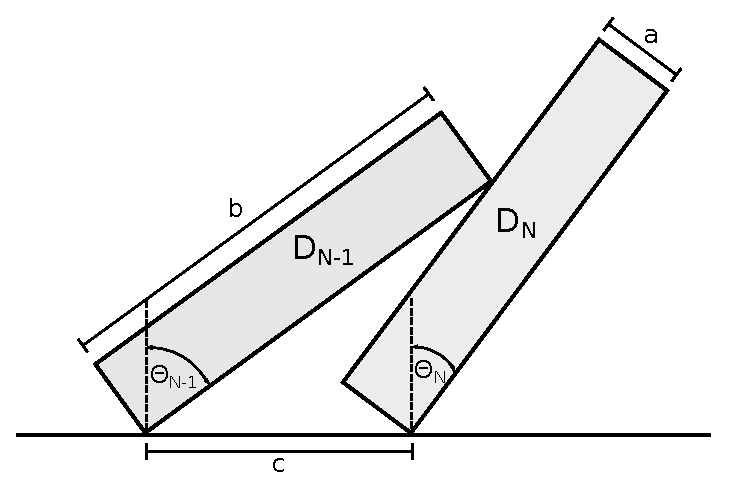
\includegraphics[width=.7\linewidth]{dominos_skizze.eps}
    \caption{Schema}
    \label{abb:1}
\end{figure}
Wir betrachten zunächst zwei aufeinanderfolgende Dominosteine wie in (\ref{abb:1}). Geht man davon aus, dass die Dominos nur rotieren können und daher nicht von ihrem Auflagepunkt abweichen, können wir die folgende trigonometrische Beziehung ableiten:
\begin{equation}
    \sin(\Theta_{N-1} - \Theta_{N}) = \frac{c}{b} \cos(\Theta_{N}) - \frac{a}{b}
    \label{eq:1}
\end{equation}
Die zeitliche Ableitung liefert schließlich:
\begin{equation}
    \dot{\Theta}_{N-1} = \left[
        1-\frac{c}{b}
        \frac{\sin{\Theta_{N}}}
        {\cos{\left(\Theta_{N-1}-\Theta_{N}\right)}}
    \right]
    \label{eq:2}
\end{equation}
Das Zeitintervall $t_N$ beschreibt die Zeit, in der ein Dominostein $D_N$ sich
aus seiner vertikalen Position herausbewegt bis er schließlich Kontakt zum
Domino $D_N$ hat. Wir erhalten genau diese Zeit durch die Energiebetrachtung.
Die Gesamtenergie $E$ des Systems setzt sich zusammen aus der kinetischen und
potentiellen Energie von allen Dominos in Bewegung.

Prinzipiell erhalten wir mit den Anfangsbedingungen bereits an dieser Stelle
eine Gleichung für $\Theta_N$. Eine analytische Lösung der Rekursionsformel ist
aufgrund der gegebenen Komplexität jedoch nicht möglich und wir entwickeln
einen numerischen Ansatz:
\begin{align}
    \cos{\Theta_i} &= U_i\cos{\Theta_N} \nonumber \\
    \sin{\Theta_i} &= V_i\sin{\Theta_N} \label{eq:3} \\
    \dot{\Theta}_i &= W_i\dot{\Theta}_N \nonumber
\end{align}
Die Koeffizienten $U_i$, $V_i$, $W_i$ werden durch wiederholte Anwendung der
Rekursionsformel (\ref{eq:1}) und (\ref{eq:2}) gewonnen. Aus (\ref{eq:3})
erhalten wir eine Gleichung für $\dot{\Theta}_N$.
\begin{equation}
    \dot{\Theta}_N = \sqrt{\frac{2E - mg
        \left( b\cos{\Theta_N} \sum_{i=1}^N U_i
        + a\sin{\Theta_N} \sum_{i=1}^N V_i \right)}
    {I \sum_{i=1}^N W_i}}
    \label{eq:4}
\end{equation}
Die Zeit $t_N$ erhalten wir nun durch einfache Integration:
\begin{equation}
    t_N = \int_0^{\Theta_C} \frac{1}{\dot{\Theta}_N} \mathrm{d}\Theta_N
    \label{eq:5}
\end{equation}
Wobei $\Theta_C$ denjenigen Winkel darstellt, bei dem ein Domino gerade mit der
oberen Kante Kontakt zum nächsten Domino hat.

Zuletzt betrachten wir die Drehimpulserhaltung in Anhängigkeit von
$\dot{\Theta}_N'$ sowie $\dot{\Theta_N''}$. Erstere Größe beschreibt die
Winkelgeschwindigkeit kurz nach dem Kontakt von $D_N$ mit $D_{N+1}$, letztere
die Geschwindikeit davor.
\begin{equation}
    I \displaystyle\sum_{i=1}^N \dot{\Theta}_N'' =
    I \displaystyle\sum_{i=1}^{N+1} \dot{\Theta}_N'
    \label{eq:6}
\end{equation}
Zusammen mit der obigen Annahme für einen numerischen Lösungsansatz erhalten
wir
\begin{equation}
    \dot{\Theta}_{N+1}' =
        \frac{\sum_{i=1}^{N} W_i''}{\sum_{i=1}^{N+1} W_i'}
        \dot{\Theta}_N''
    \label{eq:7}
\end{equation}
$W_i''$ und $W_i'$ beschreiben $W_i$ vor bzw. nach dem Kontakt.

Insgesamt können wir mithilfe von Gleichung (\ref{eq:7}) sowie $\dot{\Theta}_i
= W_i\dot{\Theta}_N$ zu allen Dominos die jeweilige Anfangswinkelgeschwindikeit
angeben. Diese Wert dienen der Berechnung der Energie $E$, welche für das
nächste Intervall $t_{N+1}$ relevant ist.
Die Gesamtzeit, welche die Kette benötigt um komplett zu fallen, erhalten wir
schließlich aus der Summation von allen Intervallen $t_i$.

Am Ende des Projektes soll eine Simulation mit genau diesem physikalischen
Hintergrund durchgeführt worden sein.


\section{Experimentelle und theoretische Vorgehensweise}
Das Projekt wird sich ungefähr gleich aus einem theoretischen, sowie einem experimentellen Teil zusammensetzen.

Im ersten Teil der Durchführung soll eine Simulation erstellt werden, in der Dominosteine mit unendlicher Haftreibung betrachtet werden. Dabei werden die physikalischen Grundlagen genutzt, welche vergangene analytische Betrachtungen bereits lieferten (Siehe dazu Literaturliste).
Das aufgestellte Modell soll am Ende Antworten auf die folgenden Fragen geben können:
Wie verhält sich die Geschwindigkeit der Dominokette bei Variation des Abstandes zwischen den Steinen? Erreicht das System immer denselben stationären Zustand, egal mit welcher Anstoßgeschwindigkeit der erste Stein fällt?

Ziel dieser Vorgehensweise ist es, zu überprüfen ob die Simulation überhaupt eine physikalische Gültigkeit besitzt. Dazu wird an dieser Stelle das erste Experiment durchgeführt.

Auf einer gummierten Unterlage – diese garantiert einen hohen Haftreibungskoeffizienten – werden Dominosteine in gleichmäßigen Abständen aufgebaut. Die Länge derselben steht zu diesem Zeitpunkt noch nicht fest, da noch nicht bekannt ist, wie lange das System braucht um eine konstante Geschwindigkeit zu erreichen.
Mithilfe einer selbstgebauten Vorrichtung, wird nun der erste Stein angestoßen und anschließend die Geschwindigkeit der Dominos mithilfe von zwei Lichtschranken bestimmt. Es werden zwei Messreihen durchgeführt.
In der ersten Reihe wird ein typischer Abstand für einen solchen Aufbau gewählt und dabei die Anstoßgeschwindigkeit variiert. Im Anschluss wird dann die Anstoßgeschwindigkeit konstant gehalten und der Abstand variiert.

Ergibt die Auswertung der erhobenen Daten, dass das aufgestellte Modell präzise genug ist, kann selbiges erweitert werden. Die Dominosteine rotieren jetzt nicht mehr um einen festen Punkt. Die Energie der Steine setzt sich zusammen aus einer Translations- sowie Rotationsbewegung. Zusätzlich wird daher der Übergang von Haft- zu Gleitreibung betrachtet.
Die Erweiterung der Simulation liefert nun einen Aufschluss darüber, wie sich die Steine auf anderen Unterlagen Verhalten.

Im letzten Teil der Durchführung werden Experimente, ähnlich wie zuvor, durchgeführt. Der Versuchsaufbau ändert sich grundsätzlich nicht, jedoch werden nun auch die Unterlagen ausgetauscht. Es erscheint sinnvoll hier von sehr glatten, bis zu sehr rauen Oberflächen alles auszuprobieren. Dieses Vorgehen ermöglicht später den Gültigkeitsbereich der gewonnenen Erkenntnisse anzugeben.

In der Auswertungsphase sollen nun die Ergebnisse diskutiert werden. Hier kann entweder angegeben werden, warum die Simulation keine realitätsnahen Ergebnisse liefert, beziehungsweise, inwiefern die Simulation noch weiter verbessert werden kann.


\section{Materialliste}
\begin{itemize}
    \item rechteckige Dominosteine, mindestens 200 Stück
    \item gummierte Unterlage, 2m lang
    \item weitere Unterlagen, alle 2m lang, z.B.
    \begin{itemize}
        \item Spiegel als glatte Oberfläche
        \item Holztisch
        \item Schleifpapier
    \end{itemize}
    \item Zwei Lichtschranken zur Zeitmessung
    \item Elektromotor zum Anstoßen des ersten Steins
    \item Computer mit Python
    \item Highspeed Kamera zur Bestimmung der Winkelgeschwindigkeit \\
\end{itemize}


\section{Zeitplan}
\begin{figure}[h!]
    \centering
    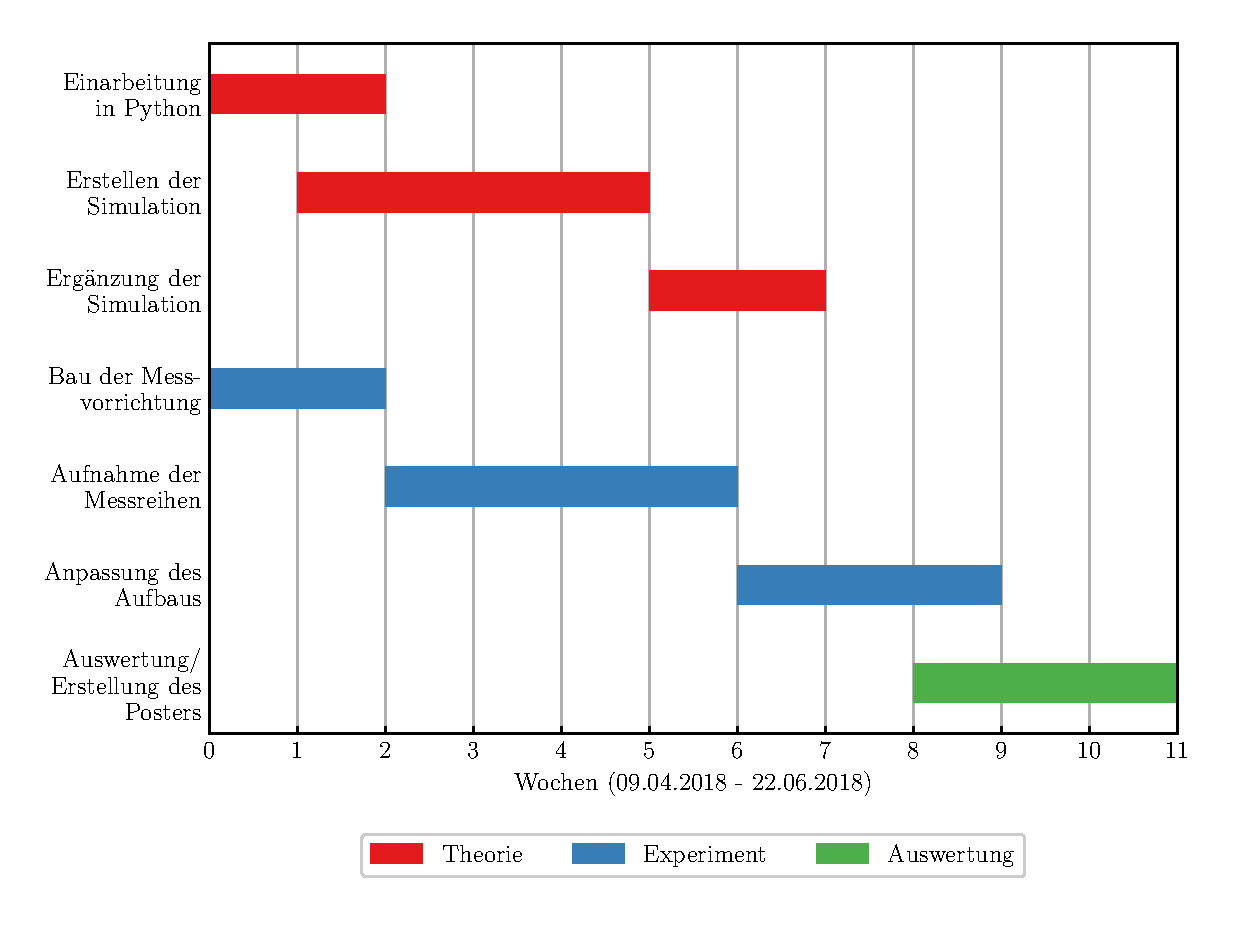
\includegraphics[width=\textwidth]{timetable.eps}
    \caption{Zeitplan}
    \label{abb:2}
\end{figure}


\section{Literaturliste}
\begin{itemize}
    \item D. E. Shaw: \emph{Mechanics of a chain of dominoes}, 1977
    \item S. Koelhoffer, C. Kuhns, K. Tsang, M. Zeitz: \emph{Falling Dominoes}, 2005 \\
\end{itemize}

\end{document}
